\documentclass[11pt]{article}

\newcommand{\wshop}{
    8
}
\newcommand{\subtitle}{
    NP
}

% Page Setup
\usepackage{geometry}
\geometry{
    a4paper,
    margin={2.5cm}
}

% Basic Packages
\usepackage{amssymb}
\usepackage{stmaryrd}
\usepackage{amsmath}
\usepackage{amsthm}
\usepackage{mathtools}
\usepackage{mathpartir}
\usepackage{enumitem}
\usepackage{mathabx}

% Font
\usepackage{charter}

% Bibliography and index
\usepackage[backend=biber, style=numeric]{biblatex}
\addbibresource{refs.bib}
\usepackage{makeidx}
\makeindex

% Colors and Graphics
\usepackage[dvipsnames, x11names]{xcolor}
\usepackage{tikz}
\usetikzlibrary{
    cd,
    fit,
    calc,
    positioning,
    arrows,
    automata,
    shapes
}
\tikzset{
    baseline = (current bounding box.center),
    every state/.append style = {
        rectangle,
        rounded corners=5pt,
		inner sep = 3pt,
		minimum size = 18pt,
		initial text = {},
        fill=Azure1
	},
	every edge/.append style = {
		->,
		>=stealth,
		bend angle=10,
		thick
	}
}
\usepackage{musicography}
\usepackage{graphicx}
\usepackage{svg}
\graphicspath{../imgs/}

% Hyperlinks
\usepackage{hyperref}
\hypersetup{
    colorlinks,
    linkcolor   = black,
    filecolor   = RubineRed,
    urlcolor    = RubineRed,
    citecolor   = RubineRed,
    pdftitle    = {Notes on Behavioural PDEs}
}
\usepackage[capitalize]{cleveref}

% Environments
\theoremstyle{theorem} % In Italics
\newtheorem{theorem}        {{\color{Purple}Theorem}}
\newtheorem{lemma}          [theorem]   {{\color{Magenta}Lemma}}
\newtheorem{proposition}    [theorem]   {Proposition}
\newtheorem{corollary}      [theorem]   {Corollary}
\newtheorem{question}                   {{\color{red}Question}}

\theoremstyle{definition} % Not in italics
\newtheorem{definition}     [theorem]   {{\color{NavyBlue}Definition}}
\newtheorem{example}        [theorem]   {{\color{ForestGreen}Example}}
\newtheorem{problem}                    {{\color{BurntOrange}Problem}}

\theoremstyle{remark} % Subdued label
\newtheorem{remark}[theorem]        {{\color{Gray}Remark}}

% (1), (2), ...
\renewcommand\labelenumi{(\theenumi)}

% Go nuts with line breaks 
\allowdisplaybreaks

%%%%%%%%%%
% MACROS %
%%%%%%%%%%

\newcommand{\op}{\mathrm{op}}               % Opposite
\newcommand{\inv}{{-1}}                     % Inverse
\newcommand{\id}{\mathsf{id}}               % Identity f(x) = x
\newcommand{\Det}{\mathrm{Det}}             % determinize
\newcommand{\Lang}{\mathcal{L}}             % Language

\newcommand{\incl}{\mathsf{incl}}           % Inclusion
\newcommand{\proj}{\mathsf{proj}}           % Projection

% Numbers and Standard notation
\newcommand{\NN}{\mathbb{N}}                % 0, 1, 2, 3, 4, ...
\newcommand{\ZZ}{\mathbb{Z}}                % ..., -2, -1, 0, 1, 2, ...
\newcommand{\QQ}{\mathbb{Q}}                % n/m for n and m in \NN and m > 0
\newcommand{\RR}{\mathbb{R}}                % real numbers
\newcommand{\pRR}{\mathbb{R}_{+}}           % positive real numbers

\newcommand{\dom}{\mathrm{dom}}             % Domain
\newcommand{\cod}{\mathrm{cod}}             % Codomain

\newcommand{\Grph}{\operatorname{Grph}}     % Graph of a function

% Transitions
\newcommand{\tr}[1]{
    \mathrel{
        \raisebox{-1pt}{
            \(\xrightarrow{#1}\)
        }
    }
}
\newcommand{\bisim}{\mathrel{\raisebox{1pt}{\(\underline{\leftrightarrow}\)}}}

% Text
\newcommand{\code}[1]{\texttt{#1}}
\newcommand{\codeblock}[1]{
    \begin{center}
        \parbox{0.8\textwidth}{
            \ttfamily
            #1
        }
    \end{center}
}

% Boolean statements
\newcommand{\OR}{~\mathrm{or}~}
\newcommand{\AND}{~\mathrm{and}~}
\newcommand{\NOT}{\mathrm{not}~}
\newcommand{\IMPLIES}{~\mathrm{implies}~}
\newcommand{\FORALL}{\mathrm{for\ all}~}
\newcommand{\EXISTS}{\mathrm{there\ exists}~}
\newcommand{\SUCHTHAT}{~\mathrm{such\ that}~}



% Title
\title{CSCI 341 Workshop \wshop}
\author{\subtitle}
% \date{
%     \today
% }

\pagestyle{empty}

\begin{document}


\maketitle

%%%%%%%%%%%%%%%%%%%%%%%%%%%%%%%%%%%%%%%%%%%%%%%%%%%%%%%%%%%%
% START OF WORK SHOP.                                      %
%%%%%%%%%%%%%%%%%%%%%%%%%%%%%%%%%%%%%%%%%%%%%%%%%%%%%%%%%%%%

\begin{problem}
    [Word Acceptance Problem for Finite Automata]
    Consider the following decision problem:
    recall that a finite automaton is a quadruple \(\mathcal A = (Q, A, \delta, F)\) with a set \(Q\) of states, a transition relation \(\delta \subseteq Q \times A \times Q\), and a set of accepting states \(F \subseteq Q\).
    The \emph{word acceptance problem for finite automata} is the decision problem
    \[
        \mathit{WAcc} = \{(\mathcal A, x, w) \mid \text{\(\mathcal A\) is a finite automaton, \(x \in Q\), and \(w \in \mathcal L(\mathcal A, x)\)}\}
    \]
    We are going to show that this language is in \(\mathsf{NP}\).
    \begin{enumerate}
        \item Start by considering the related problem 
        \[
            \mathit{DWacc} = \{(\mathcal A, x, w) \mid \text{\(\mathcal A\) is a deterministic finite automaton, \(x \in Q\), and \(w \in \mathcal L(\mathcal A, x)\)}\}
        \]
        \begin{enumerate}[label={(\alph*)}]
            \item Assume you have a class (like in Python or Java or C++) that stores an automaton and allows you to observe the set \(\delta(x, a)\) for any \(x \in Q\) and \(a \in A\).
            Write some pseudocode that decides whether \((\mathcal A, x, w) \in \mathit{DWacc}\) for any instance \((\mathcal A, x, w)\) of the problem.
            
            \item Come up with a faithful string representation of the deterministic word acceptance problem.\\
            {\footnotesize\it Hint: how would you describe a finite automaton with a basic text editor?} 

            \item Show that (the string representation of) \(\mathit{DWacc}\) is in \(\mathsf{P}\) by adapting your pseudocode from part (a) to run on a Turing machine (do you need multiple tapes?).
        \end{enumerate}

        \item Adapt your work from (1) to describe a verifier that solves \(\mathit{Wacc}\) in nondeterministic polynomial time.
        
        \item Doesn't this contradict Rice's theorem?
    \end{enumerate}
\end{problem}

\pagebreak

\begin{problem}
    \label{firstprob}
    [Graph Reachability Problem]
    A \emph{directed graph} is a pair \(\mathcal G = (X, \to)\) consisting of a set \(X\) of \emph{nodes} and a relation \({\to} \subseteq X \times X\) of \emph{edges}.
    Given nodes \(x,y \in X\), \(y\) is \emph{reachable from \(x\)} if there are \(x_1,\dots, x_n \in X\) such that 
    \[
        x \to x_1 \to x_2 \to \cdots \to x_n \to y
    \]
    Define \[
        \mathbf{DGr} = \{(\mathcal G, x, y) \mid \text{\(\mathcal G = (X, \to)\) is a directed graph and \(x,y \in X\)} \}
    \]
    Then the \emph{reachability problem} is 
    \[
        \mathit{Rch} = \{(\mathcal G, x, y) \in \mathbf{DGrph} \mid \text{\(y\) is reachable from \(x\) in \(\mathcal G\)} \} \subseteq \mathbf{DGr}
    \]
    \begin{enumerate}
        \item Write down the sets \(X\) and \(\to\) of nodes and edges in the directed graph below.
        \[
            \mathcal G = (X, \to)
            \qquad 
            \parbox{0.5\textwidth}{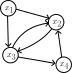
\includegraphics[scale=0.5]{digraph_1.pdf}}
        \]
        \begin{enumerate}[label={(\alph*)}]
            \item Is \((\mathcal G, x_1, x_2)\) in \(\mathit{Rch}\)?
            \item Is \((\mathcal G, x_2, x_1)\) in \(\mathit{Rch}\)?
            \item Is \((\mathcal G, x_1, x_4)\) in \(\mathit{Rch}\)?
            \item Is \((\mathcal G, x_4, x_1)\) in \(\mathit{Rch}\)?
        \end{enumerate}
        
        \item Come up with a faithful string representation of the reachability problem, and write down the string representation of \((\mathcal G, x_1, x_4)\) above.\\
        {\footnotesize\it Hint: try describing the directed graph above with a basic text editor.}

        \item Now we'll show that the reachability problem is in \(\mathsf{NP}\).
        Remember that the goal is to describe a general Turing program that either verifies or disproves that a particular instance of the problem lies in (the string representation of) \(\mathit{Rch}\) in polynomial time.
        \begin{enumerate}[label={\alph*}]
            \item Write some pseudocode that describes a nondeterministic algorithm for solving the problem. 
            What is a "guess" in this scenario?
            Write down the definition of "verification in polynomial time" and check that your pseudocode does, in fact, run in polynomial time.

            \item Now let's think about how to do this with a Turing machine.
            Describe a few different ways that you might set up the tape to store all of the necessary information about a string representation of \((\mathcal G, x, y)\) and the information you need to keep track of as the program runs. 
            Decide which one you like best as a team.

            \item Use your pseudocode in (a) to describe a Turing machine that implements your algorithm.
            Check that it runs in nondeterministic polynomial time.
        \end{enumerate}
    \end{enumerate}
\end{problem}

\pagebreak

\begin{problem}
    [Strongly Connected Problem]
    A directed graph \(\mathcal G = (X, \to)\) is \emph{strongly connected} if for any \(x,y \in X\), \(x\) is reachable from \(y\) and \(y\) is reachable from \(x\). 
    Show that the problem 
    \[
        \mathit{SCon} = \{\mathcal G \mid \text{\(\mathcal G\) is a strongly connected directed graph}\}
    \]
    is in \(\mathsf{NP}\) by cooking up a reduction \(r \colon \mathit{SCon} \preceq \mathit{Rch}\) that runs in \(\mathcal O(n^2)\)-time.
\end{problem}

\pagebreak

If you don't quite get to this problem, don't worry, we will go over it briefly in class on Friday.

\begin{problem}
    [SAT]
    The set \(\mathit{Form}\) of all \emph{(propositional) formulas} is generated by the grammar 
    \[
        F \to p \mid (F \wedge F) \mid (F \vee F) \mid (\neg F)
    \]
    where \(p \in \mathbb P\), \(\mathbb P\) is the set of \emph{basic propositional formulas}.
    An \emph{assignment} is a function \(\alpha \colon \mathbb P \to \{0,1\}\), indicating whether each basic proposition is taken to be ``false'' or ``true''.
    The \emph{truth value of a formula} is computed from an assignment \(\alpha\) recursively with the truth table below:
    \[\begin{array}{|c | c | c | c | c|}
        \hline
        \varphi_1 & \varphi_2 & \varphi_1 \wedge \varphi_2 & \varphi_1 \vee \varphi_2 & \neg \varphi_1 \\
        \hline
        1 & 1 & 1 & 1 & 0 \\
        0 & 1 & 0 & 1 & 1 \\
        1 & 0 & 0 & 1 & 0 \\
        0 & 0 & 0 & 0 & 1 \\
        \hline
    \end{array}\]
    \begin{itemize}
        \item Consider the following decision problem:
        \[
            \mathit{FTrue} = \{(\varphi, \alpha) \mid \varphi \in \mathit{Form}, \alpha \colon \{p,q,r\} \to \{0,1\}\}
        \]
        Show that (a string representation of) \(\mathit{FTrue}\) is in \(\mathsf{P}\).

        \item A formula \(\varphi \in \mathit{Form}\) is \emph{satisfiable} if there exists an assignment \(\alpha \colon \mathbb P \to \{0,1\}\) that makes \(\varphi = 1\) (i.e., true).
        We obtain the decision problem 
        \[
            \mathit{SAT} = \{\varphi \in \mathit{Form} \mid \text{\(\varphi\) is satisfiable}\}
        \]
        Use your polynomial time algorithm in the previous part to show that (a string representation of) \(\mathit{SAT}\) is in \(\mathsf{NP}\).
    \end{itemize}
    
\end{problem}


\end{document}